%Version 3 October 2023
% See section 11 of the User Manual for version history
%
%%%%%%%%%%%%%%%%%%%%%%%%%%%%%%%%%%%%%%%%%%%%%%%%%%%%%%%%%%%%%%%%%%%%%%
%%                                                                 %%
%% Please do not use \input{...} to include other tex files.       %%
%% Submit your LaTeX manuscript as one .tex document.              %%
%%                                                                 %%
%% All additional figures and files should be attached             %%
%% separately and not embedded in the \TeX\ document itself.       %%
%%                                                                 %%
%%%%%%%%%%%%%%%%%%%%%%%%%%%%%%%%%%%%%%%%%%%%%%%%%%%%%%%%%%%%%%%%%%%%%

%%\documentclass[referee,sn-basic]{sn-jnl}% referee option is meant for double line spacing

%%=======================================================%%
%% to print line numbers in the margin use lineno option %%
%%=======================================================%%

%%\documentclass[lineno,sn-basic]{sn-jnl}% Basic Springer Nature Reference Style/Chemistry Reference Style

%%======================================================%%
%% to compile with pdflatex/xelatex use pdflatex option %%
%%======================================================%%

%%\documentclass[pdflatex,sn-basic]{sn-jnl}% Basic Springer Nature Reference Style/Chemistry Reference Style


%%Note: the following reference styles support Namedate and Numbered referencing. By default the style follows the most common style. To switch between the options you can add or remove “Numbered” in the optional parenthesis. 
%%The option is available for: sn-basic.bst, sn-vancouver.bst, sn-chicago.bst%  
 
%%\documentclass[sn-nature]{sn-jnl}% Style for submissions to Nature Portfolio journals
%%\documentclass[sn-basic]{sn-jnl}% Basic Springer Nature Reference Style/Chemistry Reference Style
\documentclass[sn-mathphys-num]{sn-jnl}% Math and Physical Sciences Numbered Reference Style 
%%\documentclass[sn-mathphys-ay]{sn-jnl}% Math and Physical Sciences Author Year Reference Style
%%\documentclass[sn-aps]{sn-jnl}% American Physical Society (APS) Reference Style
%%\documentclass[sn-vancouver,Numbered]{sn-jnl}% Vancouver Reference Style
%%\documentclass[sn-apa]{sn-jnl}% APA Reference Style 
%%\documentclass[sn-chicago]{sn-jnl}% Chicago-based Humanities Reference Style

%%%% Standard Packages
%%<additional latex packages if required can be included here>

\usepackage{graphicx}%
\usepackage{multirow}%
\usepackage{amsmath,amssymb,amsfonts}%
\usepackage{amsthm}%
\usepackage{mathrsfs}%
\usepackage[title]{appendix}%
\usepackage{xcolor}%
\usepackage{textcomp}%
\usepackage{manyfoot}%
\usepackage{booktabs}%
\usepackage{algorithm}%
\usepackage{algorithmicx}%
\usepackage{algpseudocode}%
\usepackage{listings}%
\usepackage[figuresright]{rotating}
\usepackage{cuted}  % Gói cuted
\usepackage{lipsum}  % Để tạo văn bản mẫu
\usepackage{multirow}
\usepackage{booktabs}% correct bad hyphenation here
\usepackage{colortbl} 
% \usepackage{vntex} % Gói hỗ trợ font tiếng Việt
% \usepackage[T5]{fontenc} % Sử dụng font T5 cho tiếng Việt
\usepackage{graphicx}
\usepackage{hyperref}
\usepackage{multirow}
\usepackage{booktabs}% correct bad hyphenation here
\usepackage{colortbl} 
    
\usepackage{graphicx}  % Make sure to include this package in your preamble
\usepackage{subcaption} % Add this package for subfigures

%%%%

%%%%%=============================================================================%%%%
%%%%  Remarks: This template is provided to aid authors with the preparation
%%%%  of original research articles intended for submission to journals published 
%%%%  by Springer Nature. The guidance has been prepared in partnership with 
%%%%  production teams to conform to Springer Nature technical requirements. 
%%%%  Editorial and presentation requirements differ among journal portfolios and 
%%%%  research disciplines. You may find sections in this template are irrelevant 
%%%%  to your work and are empowered to omit any such section if allowed by the 
%%%%  journal you intend to submit to. The submission guidelines and policies 
%%%%  of the journal take precedence. A detailed User Manual is available in the 
%%%%  template package for technical guidance.
%%%%%=============================================================================%%%%

%% as per the requirement new theorem styles can be included as shown below
%\theoremstyle{thmstyleone}%
\newtheorem{theorem}{Theorem}%  meant for continuous numbers
%%\newtheorem{theorem}{Theorem}[section]% meant for sectionwise numbers
%% optional argument [theorem] produces theorem numbering sequence instead of independent numbers for Proposition
\newtheorem{proposition}[theorem]{Proposition}% 
%%\newtheorem{proposition}{Proposition}% to get separate numbers for theorem and proposition etc.

%\theoremstyle{thmstyletwo}%
\newtheorem{example}{Example}%
\newtheorem{remark}{Remark}%

%\theoremstyle{thmstylethree}%
\newtheorem{definition}{Definition}%

\raggedbottom
%%\unnumbered% uncomment this for unnumbered level heads
\usepackage{amsmath}
\usepackage{amsfonts}

\begin{document}

\title[Article Title]{A Hybrid Deep Learning Model for Solar Energy Forecasting on Edge Computing}

%%=============================================================%%
%% GivenName	-> \fnm{Joergen W.}
%% Particle	-> \spfx{van der} -> surname prefix
%% FamilyName	-> \sur{Ploeg}
%% Suffix	-> \sfx{IV}
%% \author*[1,2]{\fnm{Joergen W.} \spfx{van der} \sur{Ploeg} 
%%  \sfx{IV}}\email{iauthor@gmail.com}
%%=============================================================%%

\author*[1,2]{\fnm{First} \sur{Author}}\email{iauthor@gmail.com}

\author[2,3]{\fnm{Second} \sur{Author}}\email{iiauthor@gmail.com}
\equalcont{These authors contributed equally to this work.}

\author[1,2]{\fnm{Third} \sur{Author}}\email{iiiauthor@gmail.com}
\equalcont{These authors contributed equally to this work.}

\affil*[1]{\orgdiv{Department}, \orgname{Organization}, \orgaddress{\street{Street}, \city{City}, \postcode{100190}, \state{State}, \country{Country}}}

\affil[2]{\orgdiv{Department}, \orgname{Organization}, \orgaddress{\street{Street}, \city{City}, \postcode{10587}, \state{State}, \country{Country}}}

\affil[3]{\orgdiv{Department}, \orgname{Organization}, \orgaddress{\street{Street}, \city{City}, \postcode{610101}, \state{State}, \country{Country}}}

%%==================================%%
%% Sample for unstructured abstract %%
%%==================================%%

\abstract
{
\indent In the domain of sustainable energy management for Internet of Things (IoT) infrastructures, precise long-term solar energy prediction is of paramount importance. This paper introduces a hybrid deep learning architecture that integrates Temporal Convolutional Networks (TCNs) with Gated Recurrent Units (GRUs), specifically optimized for execution on edge computing devices characterized by restricted computational capabilities. The framework capitalizes on the TCN's proficiency in capturing extensive temporal dependencies alongside the GRU's adeptness at efficiently processing sequential data. To further augment performance, optimization methodologies such as Neural Architecture Search (NAS), model pruning, and quantization are implemented, yielding substantial reductions in both model size and complexity. The proposed framework is assessed against two benchmark datasets, namely the competition dataset and GEFCom2014, revealing enhanced accuracy in comparison to leading forecasting models. In particular, it accomplishes a Mean Squared Error (MSE) of 0.0051 on long-range forecasts, while preserving computational efficiency appropriate for edge devices. These findings indicate that the model is highly suitable for real-time IoT-driven solar energy applications.
}

%%================================%%
%% Sample for structured abstract %%
%%================================%%

% \abstract{\textbf{Purpose:} The abstract serves both as a general introduction to the topic and as a brief, non-technical summary of the main results and their implications. The abstract must not include subheadings (unless expressly permitted in the journal's Instructions to Authors), equations or citations. As a guide the abstract should not exceed 200 words. Most journals do not set a hard limit however authors are advised to check the author instructions for the journal they are submitting to.
% 
% \textbf{Methods:} The abstract serves both as a general introduction to the topic and as a brief, non-technical summary of the main results and their implications. The abstract must not include subheadings (unless expressly permitted in the journal's Instructions to Authors), equations or citations. As a guide the abstract should not exceed 200 words. Most journals do not set a hard limit however authors are advised to check the author instructions for the journal they are submitting to.
% 
% \textbf{Results:} The abstract serves both as a general introduction to the topic and as a brief, non-technical summary of the main results and their implications. The abstract must not include subheadings (unless expressly permitted in the journal's Instructions to Authors), equations or citations. As a guide the abstract should not exceed 200 words. Most journals do not set a hard limit however authors are advised to check the author instructions for the journal they are submitting to.
% 
% \textbf{Conclusion:} The abstract serves both as a general introduction to the topic and as a brief, non-technical summary of the main results and their implications. The abstract must not include subheadings (unless expressly permitted in the journal's Instructions to Authors), equations or citations. As a guide the abstract should not exceed 200 words. Most journals do not set a hard limit however authors are advised to check the author instructions for the journal they are submitting to.}

\keywords{Internet of Things, Solar Energy Forecasting, Hybrid Deep Learning, Edge Computing.}

%%\pacs[JEL Classification]{D8, H51}

%%\pacs[MSC Classification]{35A01, 65L10, 65L12, 65L20, 65L70}

\maketitle

\section{Introduction}\label{sec1}
The growing global reliance on sustainable energy sources underscores the pivotal role of solar energy within today's energy landscape. Precise forecasting of solar energy generation is crucial for enhancing the energy management of solar PV systems \cite{venkatesan2024integrating}. The integration of data-gathering IoT (Internet of Things) systems opens accurate long-term solar power output prediction to boost the system's reliability and efficiency \cite{kazmi2023iot}, \cite{feng2022multi}. With the swift advancement of AI applications in forecasting, machine learning and deep learning models have significantly elevated solar power output prediction capabilities beyond traditional techniques. These innovative solutions offer remarkable scalability and enhanced performance for the planning and operation of distributed systems\cite{hu2024short}. The solar power forecasting challenge falls under the umbrella of time series forecasting problems, necessitating high precision in both short-term and long-term predictions. Some deep learning models, including Temporal Convolution Networks (TCN), have managed to tackle the issue of predicting solar power output from sequential data. Unfortunately, they struggle with longer sequences due to memory constraints and training speed \cite{cheng2024solar}. Moreover, TCN’s memory constraints limit its capacity to retain long-term information \cite{ferkous2024novel}. However, \cite{tamil2023solar} gets that dilated convolutions in TCN can find long-term dependencies in multivariate time series with featured processing as the time series gets longer. The gated recurrent unit (GRU) is helpful because it has an internal memory and a gating mechanism that lets it handle sequential data well. This makes prediction performance better. Hence, we propose an innovative hybrid architecture of TCN and GRU (called TGNet) to use long-term and large-scale solar power forecasting by merging both frameworks. Using TCN's feature extraction functions, the proposed model creates compressed feature vectors. GRU then uses these to make predictions that lower computational parameters, matrix size, and GRU nodes so that the architecture can be used on edge devices with limited resources. We use a neural architecture search (NAS)-based parameter optimization, prunning and quantization methods that have been added to the proposed model to make it faster and more accurate at making predictions. Experimental results were executed on Alibaba Competitive dataset and GEFCom 2014, showcasing comprehensive benchmarking against other recent studies and demonstrating superior outcomes. The primary contributions are highlighted below.

\begin{itemize}
    \item Created a hybrid TCN-GRU model (TGNet) for solar energy forecasting that makes low computational complexity while ensuring high accuracy for deployment on edge computing. 
    \item Implemented optimization strategies via neural architecture search, quantization, and neuron pruning to refine model performance. 
    \item Assessed and validated the performance on published experimental datasets, revealing superior results relative to other authors' state-of-the-art models.
\end{itemize}
 
\section{Related Work}\label{sec2}
In time series forecasting, models like Informer, TimesNet, Autformer, Non-stationary Transformer, DLinear, and GRU-XGBoost have been used for various purposes. Each model presents distinct advantages and disadvantages, especially in resource-limited and real-time settings. The Informer model provides long sequence forecasting with a ProbSparse self-attention mechanism, optimizing computation and memory. Its generative decoder enhances inference speed, which is crucial for latency-sensitive edge computing. However, the Informer struggles with non-stationary data, impacting accuracy in real-world scenarios \cite{zhou2021informer}. The TimesNet effectively captures temporal patterns, which is beneficial for real-time analysis in edge computing. However, It may lack specific optimizations for constrained edge environments \cite{wu2022timesnet}. By combining TCNs and seasonal-trend decomposition, Autformer makes long-term sequence prediction better, which also improves performance. However, its complexity can lead to higher computational overhead, complicating deployment on limited-resource edge devices  \cite{fan2023tedformer}. The nonstationary transformer model effectively manages non-stationarity with series rationalization and de-stationary attention, enhancing predictability. It significantly lowers mean squared error (MSE) across transformer models, making it reliable for dynamic environments. However, the complexity of managing non-stationarity may increase computational demands, posing challenges in edge computing \cite{liu2022non}. DLinear model is lightweight and efficient, ideal for resource-constrained edge computing. However, they might need to capture complex temporal dependencies, potentially hindering forecasting accuracy effectively.\\ 
In the domain of solar energy forecasting, hybrid deep learning models have shown significant promise in enhancing predictive accuracy and efficiency. The GRU-XGBoost model, the hybrid approach, combines GRU for temporal dependencies with XGBoost for non-linear relationships, providing balanced time series forecasting. Its nature is advantageous for edge computing, delivering strong predictions with lower computational costs. However, the model's integration complexity might hinder deployment and maintenance on edge devices, where simplicity is preferred \cite{wu2021edgelstm}. The NARX-LSTM model combines the nonlinear autoregressive with exogenous inputs (NARX) model and long short-term memory (LSTM) networks to predict daily solar irradiance. This model effectively handles non-linear relationships and long-term dependencies, achieving a mean absolute error and a root mean square error (RMSE) outperforming other benchmark models in accuracy \cite{okieh2024enhanced}. A predictive model for photovoltaic (PV) power utilizing the TCN and White Shark Optimization (WSO) algorithm enhances performance through feature selection based on the maximal information coefficient (MIC), thereby increasing the accuracy and reliability of PV power output predictions across various PV systems \cite{lin2024hybrid}. The CNN-LSTM model, integrated with variational mode decomposition (VMD), has been applied for short-term PV power forecasting. This hybrid model does a better efficiency than other deep learning models at capturing both temporal and spatial dependencies, which makes solar power predictions more accurate \cite{lakhdar_nadjib_boucetta__2024}. Another study created a hybrid model that combined singular spectrum analysis (SSA), CNNs, and LSTMs. This model did better at short-term solar power forecasting, especially in greenhouse environments \cite{venkateswaran2024efficient}. The BiLSTM-GRU model, which incorporates dropout techniques, has been shown to outperform other models in predicting solar irradiance. This model effectively captures multivariate data dependencies, achieving low RMSE and MAE values, indicating high prediction accuracy \cite{michael2024cohesive} . A 1D CNN-GRU model has been developed for short-term solar PV power forecasting. This model combines the feature extraction capability of CNNs with the forecasting accuracy of GRUs. It has the lowest RMSE across all seasons and is more accurate and efficient at training than other models\cite{venkateswaran2024efficient}.
The hybrid TCN-GRU model has been used for various purposes. In \cite{hao2021hybrid}, the authors created a powerful hybrid TCN-GRU model for predicting traffic flow. TCN is used to extract both spatial and temporal features from raw data effectively, and then GRU is used to capture long-term temporal dependencies for accurate predictions accurately. This proposed model showcased exceptional performance, surpassing baseline models such as LSTM, ARIMA, and SVM in prediction accuracy. In \cite{li2021multi} crafted a cutting-edge multi-step wind speed prediction model employing a TCN-GRU hybrid. TCN was instrumental in capturing the complex features of wind speed time-series data, and GRU expertly managed multi-step forecasting. In \cite{zhu2021hybrid} adopted a comparable strategy to forecast PM2.5 concentration using environmental time-series data.\\ 
The deployment of deep learning for solar energy forecasting on edge devices is a novel research area with limited studies. The authors in \cite{Kumar2018} highlighted machine learning frameworks like TensorFlow Lite and PyTorch Mobile for lightweight development on edge devices. The authors in \cite{Chen2020} introduced a federated learning framework for IoT, facilitating model training without raw data sharing, thus enhancing privacy and bandwidth. The authors in \cite{GruossoGajani2022} improved models for predicting solar energy by looking at how quantization and pruning affect edge deployment with limited resources. In \cite{Li2021} presented practical strategies for optimizing deep learning models for low-power IoT devices, ensuring efficient edge inference. The authors in \cite{Tran2022} studied how deep learning with quantization can be used to predict the output of photovoltaic panels, tackling the problematic issues of deploying complex models on edge devices.\\ 
According to the survey mentioned above, there is currently no comprehensive research on solar energy forecasting that includes both short-term and long-term perspectives. Several hybrid architectures have been proposed that mainly target one of the environmental time series data. Furthermore, the objective of implementing the model on edge computing has not been specified. Hence, our investigation will tackle the current shortcomings and overcome the obstacles related to the accuracy and complexity of this approach to deploy the framework on limited resource edge devices.

\section{Proposed Model}\label{sec3}
Figure \ref{fig:overview} presents the main components and their interconnections within the proposed hybrid deep learning model for long-term solar energy forecasting on edge computing devices. The model is designed to efficiently process multivariate time-series data, capturing both short-term and long-term temporal dependencies while being optimized for deployment on edge devices with limited computational resources. The key blocks are outlined as follows.
\begin{figure}[htbp]
  \centering
  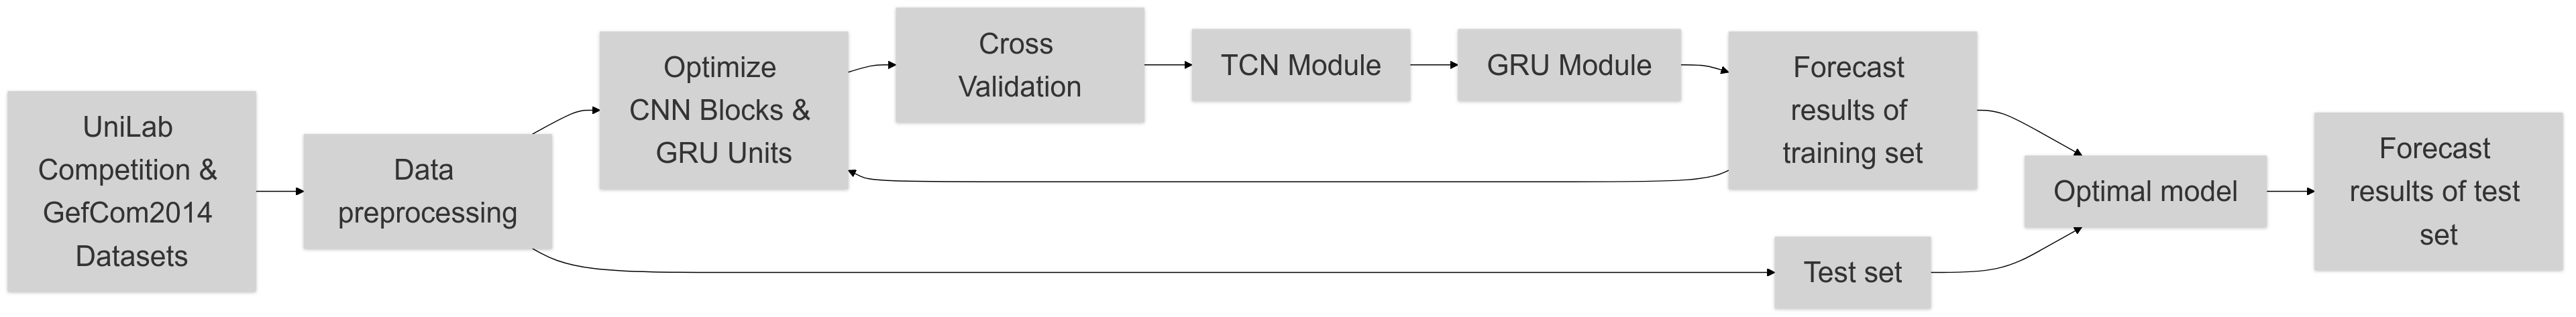
\includegraphics[width=1.0\textwidth]{overviewv2.png}
  \caption{Main diagram blocks of the proposed forecasting model}
  \label{fig:overview}
\end{figure}

Input Data: Historical solar energy generation data and meteorological characteristics, including sun irradiance, temperature, and wind velocity, are input data for the forecasting model.

Data Preprocessing: The initial dataset is cleaned, normalized, and transformed to handle missing data, noise, and feature scaling to ensure its suitability for the neural network's learning mechanisms.

Neural Architecture Search (NAS) System: The NAS framework autonomously finds and builds the best neural network architecture, improving model design for predictive performance and edge deployment computing efficiency.

Data Splitting: The dataset is split into a training set for parameter estimation and a testing set for an impartial evaluation of the model's predicted performance on unknown data.

Model Training: The TCN module extracts important features from multivariate time-series data. At the same time, the Dense Layer prepares them for a GRU module, which emphasizes temporal dependencies and produces a dense layer that predicts solar energy generation.

Cross-validation on the training dataset helps to reduce overfitting, and testing on the validation set helps to gauge predictive accuracy in model evaluation. Improved models are then deployed on edge devices for real-time forecasting.


\subsection{Mathematical Descriptions}
To create an effective solar power prediction system, we treat it as a machine learning challenge with a multivariate time series input and a predicted power output time series. Figure \ref{fig:overview} illustrates the model's input, which includes solar power output and meteorological data. The input data undergoes preprocessing, and then the NAS system identifies the best architecture, splitting the data into training and test sets. The training set includes a TCN module from NAS, Dense, GRU, and another Dense class. Model evaluation occurs through cross-validation on the training set, facilitating the selection of the best model. The optimal model is then tested on the test set, comparing predicted results to actual values for performance assessment. Cross-validation iterations enhance the model and fine-tune parameters for superior predictive accuracy.


Specifically, the input of the problem is defined as follows:
\begin{equation}
\mathbf{X} = \{\mathbf{x}_1, \mathbf{x}_2, ..., \mathbf{x}_T\}, 
\end{equation}

Where $\mathbf{X}$ represents the multivariate input time series, consisting of data points from \(x_1\) to \(x_T\). Each \(x_t\) is a feature vector at time step \(t\), containing variables that influence solar energy production, such as solar radiation, temperature, and wind speed.
\begin{equation}
\mathbf{Y} = \{y_{T+1}, y_{T+2}, ..., y_{T+H}\},
\end{equation}

Where $\mathbf{Y}$ denotes the time series of solar energy output that we aim to predict, from \(y_{T+1}\) to \(y_{T+H}\). Each \(y_t\) is the energy output value at time step \(t\), and \(H\) is the prediction horizon, indicating the number of future time steps we want to forecast. Our objective is to establish a precise mapping function:

\begin{equation}
\mathbf{f}: \mathbb{R}^{T \times d} \rightarrow \mathbb{R}^H
\end{equation}

f is a mapping function from the input space \(\mathbb{R}^{T \times d}\) (where \(T\) is the number of time steps and \(d\) is the number of features) to the output space \(\mathbb{R}^H\) (the number of time steps to predict). The goal of the model is to find an accurate mapping function that can predict Y from X, or:

\begin{equation}
\mathbf{Y} \approx \mathbf{f}(\mathbf{X}).
\end{equation}

The model strives to make the predicted values \(f(X)\) as close as possible to the actual values Y. This means that the closer the predicted solar energy output \(f(X)\) is to the actual value, the more accurate the model is. 

\subsection{The proposed model architecture}
 The architecture of a TCN confidently comprises several 1D convolution layers with progressively more significant expansion coefficients. A nonlinear activation function (ReLU) that can also include a normalization layer (such as batch normalization) follows each concatenation layer. A TCN is constructed with residual blocks, each featuring two layers of dilated volumes that utilize shared weighting parameters. This design empowers TCN to possess an extensive receptive field and the capability to master intricate features while efficiently preserving a relatively compact number of parameters.

\begin{figure}[htbp]
  \centering
  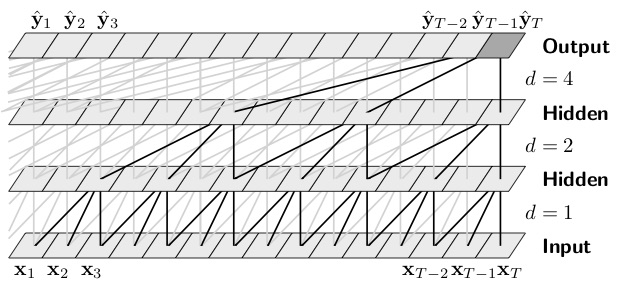
\includegraphics[width=0.45\textwidth]{tcn3d.jpg}
  \caption{The relationships in input multivariate data and vector-embedded connections.}
  \label{fig:tcn3d}
\end{figure}

The 1D dilated convolution operation in TCN is defined as follows:
\begin{equation}
y[t] = \sum_{k=0}^{K-1} w_k \cdot x[t - d \cdot k]
   \end{equation}

Where \(y [t]\) represents the output at time\(t\); \(x [t]\) denotes the input at time\(t\); \(w_k\) signifies the weight of the filter (kernel) at position\(k\); \(K\) stands for the size of the kernel. \(d\) indicates the expansion coefficient. 
The expansion coefficient \(d\) empowers the kernel to remove several input elements, significantly enhancing the model's receptive field. The receptive field of a TCN with \(L\) classes and a kernel size of \(K\) is determined as follows:
\begin{equation}
\text{ReceptiveField} = 1 + \sum_{l=0}^{L-1} (K - 1) \cdot d_l
\end{equation}
This represents the range of input time steps that influence a particular output time step in the network. In the context of a TCN, the receptive field determines the model’s ability to capture long-term dependencies within the time series data. This formula calculates the total receptive field of the TCN by summing the contributions of each layer. The dilation rate $(d_l)$ lets the network exponentially expand the receptive field without expanding the number of layers. This makes it possible to efficiently capture long-range dependencies. Residual connections in TCN are calculated in the following manner.
\begin{equation}
o[t] = Activation(x[t] + F(x[t]))    
\end{equation}
This equation describes the residual connection within the TCN. By adding the input \( x[t] \) to the output of the convolutional layers \( F(x[t]) \), the network facilitates the flow of information and mitigates the vanishing gradient problem, thereby enhancing training efficiency and model performance.
In which, \(o[t]\) represents outputs of residual blocks at time \(t\). \(x[t]\) represents inputs of residual blocks at time \(t\). \(F(x [t])\) represents the output of the convolution classes within the residual block. Equations (6) and (7) describe the architecture of the TCN, highlighting the calculation of the receptive field and the implementation of residual connections to enhance model training and performance. 

\begin{figure}[htbp]
  \centering
  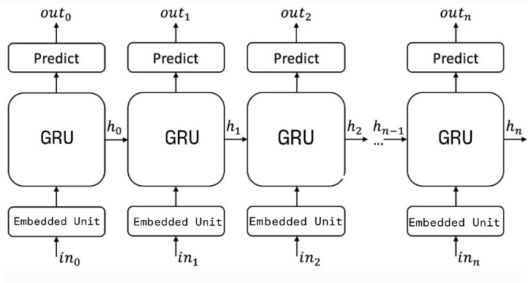
\includegraphics[width=0.4\textwidth]{gru.jpg}
  \caption{ The GRU process diagram for connecting the characteristic vectors.}
  \label{fig:gru}
\end{figure}

The proposed TCN-GRU architecture captures time-series characteristics while effectively modeling the time dependencies. It confidently incorporates the dilated convolution classes as follows.
     \begin{equation}
    \mathbf{h}_t^{(l)} = \sigma \left( \sum_{k=0}^{K-1} \mathbf{W}_k^{(l)} \cdot \mathbf{x}_{t-d \cdot k}^{(l-1)} + \mathbf{b}^{(l)} \right)    
    \end{equation}
Where, $\mathbf{h}_t^{(l)} \in \mathbb{R}^{n_l}$ is output of the class $l$ at the time $t$. $\mathbf{x}_t^{(l-1)}$ is input of class $l$ (output of the previous), with $\mathbf{x}_t^{(0)} = \mathbf{x}_t$. $K$ is kernel size.
    $d$ is dilation rate;$n_l$ is number of filters in the class $l$.
    $\mathbf{W}_k^{(l)} \in \mathbb{R}^{n_l \times n_{l-1}}$ và $\mathbf{b}^{(l)} \in \mathbb{R}^{n_l}$ is weight factor and bias factor of the class $l$.
    $\sigma$ is activation functions(ReLU, sigmoid, tanh). The dimension reduction is executed by Pooling unit. Then, GRU updates the hidden status as equation below. 
\begin{equation}
\mathbf{r}_t = \sigma(\mathbf{W}_r \cdot [\mathbf{h}_{t-1}, \mathbf{z}_t] + \mathbf{b}_r) 
\end{equation}
\begin{equation}
\mathbf{u}_t = \sigma(\mathbf{W}_u \cdot [\mathbf{h}_{t-1}, \mathbf{z}_t] + \mathbf{b}_u) 
\end{equation}
\begin{equation}
\tilde{\mathbf{h}}_t = \tanh(\mathbf{W}_h \cdot [\mathbf{r}_t \odot \mathbf{h}_{t-1}, \mathbf{z}_t] + \mathbf{b}_h) 
\end{equation}
\begin{equation}
\mathbf{h}_t = (1 - \mathbf{u}_t) \odot \mathbf{h}_{t-1} + \mathbf{u}_t \odot \tilde{\mathbf{h}}_t
\end{equation}
Where, $\mathbf{z}_t$ is feature vector; $\mathbf{r}_t, \mathbf{u}_t$ represents to reset and update ports; $\tilde{\mathbf{h}}_t$ is the potential hidden state variable.
$\mathbf{h}_t$ is hidden state of GRU at the time $t$.  
Equations (8) to (12) elaborate on the GRU unit’s internal mechanisms, including the reset and update gates, and the computation of the hidden states, which collectively enable the model to capture and retain long-term dependencies in sequential data effectively.

\subsection{Optimization Process}
 To deploy the proposed model on resource-constrained edge devices, we use the NAS based on reinforcement learning algorithm to optimize the proposed model. Some basic computational steps are presented below.
To enhance the TCN efficiency, we adopt the MobileNet (MBConv) block. MBConv features depthwise separable convolution, which significantly reduces the number of parameters and computational costs compared to conventional convolution while maintaining high performance. We tune the key hyperparameters of the MBConv block, including the number of filters, kernel size, and dilation ratio, to determine the optimal MBConv configuration for this problem. After determining the optimal hyperparameters for the model, the next phase involved designing, searching for optimal architecture, and performing pruning and quantization. Optimizing the neural network architecture plays a crucial role in efficient deployment on edge devices, where computational resources are often limited. In this subsequent stage, we experimented with employing a Neuron Architecture Search algorithm. The search space encompassed the number of filters in each Conv1D layer (ranging from 16 to 128 with a step size of 16), the kernel size of the DepthwiseConv1D layers (from 3 to 7 with a step size of 2), the number of units in the GRU layer (from 10 to 50 with a step size of 10), and the learning rate (selected from 1e-2, 1e-3, 1e-4). The search process was conducted with a maximum of 10 epochs for each model, and the Hyperband factor was set to 3. Upon completion of the search, the best model was selected based on its loss function value on the validation set. 

\section{Experimental results and Discussions}\label{sec4}

This section details the experimental setup used to evaluate the performance and efficiency of the proposed TGNet solar forecasting model. The main objective of this study is to develop an accurate and efficient solar forecasting model suitable for deployment on edge devices in IoT systems. Therefore, experimental scenarios are designed to evaluate the model on several aspects, including customizability, performance compared to other forecasting methods, and the impact of optimization techniques.
\subsection{Datasets and preprocessing}
\paragraph{Competition Dataset}The first dataset is the Competition Dataset from the UNiLAB Track 3 algorithm competition, Renewable Energy Generation Prediction organized by Alibaba, which includes a 300-day history of environmental information related to solar energy production at the same location. The dataset used in the study consists of 4500 records, representing information on factors affecting solar energy production. Each record contains data for a specific hour of the day, represented by two columns, "Day" and "Hour", with the data type of integer (int64). Besides time information, the dataset also records wind direction ("Dir") and wind speed ("Spd"), which are two important factors affecting the performance of solar energy systems, along with temperature ("Temp"). The "Radiation" column records the level of solar radiation, which is a direct determinant of solar energy production. This dataset can be accessed at \href{https://github.com/xuyaojian123/solar-production-foreasting}{https://github.com/xuyaojian123/solar-production-foreasting}.
\paragraph{GEFCom2014} The second dataset is taken from the Solar folder of the Global Energy Forecasting Competition 2014 (GEFCom2014). This folder contains hourly data from three solar farms (referred to as Zone 1, Zone 2, and Zone 3) located in a specific region of Australia. GEFCom14 provides 12 weather variables and their corresponding hourly solar energy production. The GEFCom2014 dataset is available at \href{https://blog.drhongtao.com/2017/03/gefcom2014-load-forecasting-data.html}{https://blog.drhongtao.com/2017/03/gefcom2014-load-forecasting-data.html}.\\
For each dataset, the raw data is preprocessed to address missing and noisy data and normalize the data to the same range. In the data preprocessing stage, first, the raw data from three solar farms ("farm1", "farm2", "farm3") are loaded and unnecessary columns are removed. Then, the "TIMESTAMP" column is converted to date and time format and set as the index for each dataset.
Next, the data is normalized using the StandardScaler method to bring the variables into the same range, which improves the performance of the machine learning model. The class weight function is used to calculate the weight for each data sample to increase the influence of low-energy output samples during training.
The data is then converted to a time series format with a fixed window length. Finally, the data is divided into a training set, a validation set, and a test set in a ratio of 70:15:15 for training and evaluation of the model. The data is then divided into a training set, a validation set, and a test set in a ratio of 70:15:15, ensuring that the model is trained on a sufficiently large portion of the data, hyperparameters are tuned on an independent dataset, and performance is evaluated on an entirely resulted dataset.



% \begin{table*}[ht]
%     \centering
%     \caption{Kiến trúc mô hình TCN-GRU}
%     \begin{tabular}{l|l|l}
%         \toprule
%         \textbf{Lớp} & \textbf{Parameters} & \textbf{Output} \\
%         \midrule
%         Input Layer & (window\_size, num\_features) & (window\_size, num\_features) \\
%         \midrule
%         \multicolumn{3}{c}{\textbf{Khối TCN}} \\
%         \midrule
%         Conv1D (Block 1) & filters=13, kernel\_size=1, padding="causal", activation='relu' & (window\_size, 13) \\
%         BatchNormalization (Block 1) & - & (window\_size, 13) \\
%         DepthwiseConv1D (Block 1) & kernel\_size=3, dilation\_rate=1, activation='relu', padding='same' & (window\_size, 13) \\
%         BatchNormalization (Block 1) & - & (window\_size, 13) \\
%         Dropout (Block 1) & rate=0.2 & (window\_size, 13) \\
%         \midrule
%         Conv1D (Block 2) & filters=13, kernel\_size=1, activation='relu', padding="causal" & (window\_size, 13) \\
%         BatchNormalization (Block 2) & - & (window\_size, 13) \\
%         DepthwiseConv1D (Block 2) & kernel\_size=3, dilation\_rate=2, activation='relu', padding='same' & (window\_size, 13) \\
%         BatchNormalization (Block 2) & - & (window\_size, 13) \\
%         Dropout (Block 2) & rate=0.2 & (window\_size, 13) \\
%         \midrule
%         % Lặp lại cho các khối 3, 4, 5
%         \multicolumn{3}{c}{ ... } \\
%         \midrule
%         \multicolumn{3}{c}{\textbf{Khối GRU}} \\
%         \midrule
%         Dense & units=predict\_horizon & (window\_size, predict\_horizon) \\
%         GRU & units=predict\_horizon & (window\_size, predict\_horizon) \\
%         Dropout & rate=0.2 & (window\_size, predict\_horizon) \\
%         Dense (Output Layer) & units=predict\_horizon, activation='linear' & (window\_size, predict\_horizon) \\
%         \bottomrule
%     \end{tabular}
% \end{table*}

\subsection{Evaluated metrics}
To evaluate the performance of the proposed model, the main performance evaluation parameters are listed below. 
The following formula presents MSE (Mean Squared Error). 
\begin{equation}
MSE = \frac{1}{N} \sum_{i=1}^{N}(y_i - \hat{y}_i)^2,
\end{equation}
Where $y_i$ is the actual value, $\hat{y}_i$ is the predicted value, and $N$ is the number of samples. MSE measures the mean square of the deviation between the predicted value and the actual value. It is sensitive to outliers and gives greater weight to large errors. A low MSE value indicates that the model is capable of predicting accurately, but it should be noted that MSE has units of the square of the original unit. The following formula presents MAE (Mean Absolute Error).
   \begin{equation}
   MAE = \frac{1}{N} \sum_{i=1}^{N} |y_i - \hat{y}_i|.
   \end{equation}
  MAE measures the average magnitude of the prediction error and is less sensitive to outliers than RMSE. A low MAE indicates a model with good overall accuracy. $R^2$ score (coefficient of determination) is presented as.
   \begin{equation}
   R^2 = 1 - \frac{\sum_{i=1}^{N} (y_i - \hat{y}_i)^2}{\sum_{i=1}^{N} (y_i - \bar{y})^2},
   \end{equation}
  Where $\bar{y}$ is the mean value of $y_i$. The $R^2$ score evaluates how well the model fits the data and shows how much of the variation in the dependent variable the model can account for. The closer the $R^2$ score is to 1, the better the model fits the data.
Formulas (13) to (15) introduce the evaluation metrics used to assess the model’s predictive performance. MSE and MAE provide quantitative measures of prediction error, with MSE emphasizing larger errors, while MAE offers a more interpretable average error magnitude. The \( R^2 \) score complements these by indicating the proportion of variance explained by the model, thereby offering a holistic view of the model’s accuracy and reliability in forecasting solar energy output. These mathematical formulations underpin the model’s capability to accurately predict solar power generation by effectively capturing temporal dependencies and optimizing performance through robust evaluation metrics.

\subsection{Experimental scenarios}
To assess the performance of the proposed model, experiments were conducted with four solar energy forecasting cases constructed using the Competition and GEFCom2014 datasets: 15 steps (one day), 45 steps (three days), 90 steps (six days), and 150 steps (ten days). This setup adheres to the definition of long-term forecasting. The experiments were executed in a Python 3.10 environment on an RTX A4000 GPU. To ensure the reliability of the experimental results, all tests were performed under identical operational conditions. The experimental scenarios were designed to evaluate the proposed model comprehensively.\\
Performance Comparison. This experiment is used to compare the forecasting performance of the model with other models across the three datasets. The evaluation metrics are RMSE, MAE, and the $R^2$ score against other state-of-the-art forecasting models.\\
Optimization Evaluation. This scenario focuses on assessing the impact of the proposed optimization techniques over the proposed model, including optimized convolution blocks, neural architecture search, quantization, and neuron pruning techniques to reduce the model's size and complexity.\\
 Sensitivity Analysis. The objective of this experimental scenario is to evaluate the sensitivity of the proposed model facing changing input factors and hyperparameters (input sequence length and model hyperparameters). We fine-tune key hyperparameters of the model (e.g., number of layers, number of neurons, learning rate) to identify optimal configurations for forecasting performance. By analyzing the results (RMSE, MAE, $R^2$ score) obtained from adjusting these factors, we can determine the most critical factors influencing the model's performance and identify the optimal configuration for the proposed model.

\subsection{Results and Discussions}
The parameter tuning for our proposed model is compared with the original model shown in Table \ref{t1} and the predicted parameters in Table \ref{t2}.

\begin{table*}[ht!]
    \centering
    \caption{TCN-GRU Model Architecture}
    \resizebox{0.9\textwidth}{!}{
    \begin{tabular}{|l|l|l|}
        \toprule
        \textbf{Layer} & \textbf{Parameters} & \textbf{Output Shape} \\
        \midrule
        Input Layer & (window\_size, num\_features) & (window\_size, num\_features) \\
        \midrule
        \multicolumn{3}{|c|}{\textbf{TCN Block}} \\
        \midrule
        Conv1D (Block 1) & filters=num\_features, kernel\_size=3, dilation\_rate=1, activation='relu', padding='causal' & (window\_size, num\_features) \\
        Conv1D (Block 2) & filters=num\_features, kernel\_size=3, dilation\_rate=2, activation='relu', padding='causal' & (window\_size, num\_features) \\
        Conv1D (Block 3) & filters=num\_features, kernel\_size=3, dilation\_rate=4, activation='relu', padding='causal' & (window\_size, num\_features) \\
        Conv1D (Block 4) & filters=num\_features, kernel\_size=3, dilation\_rate=8, activation='relu', padding='causal' & (window\_size, num\_features) \\
        Conv1D (Block 5) & filters=num\_features, kernel\_size=3, dilation\_rate=16, activation='relu', padding='causal' & (window\_size, num\_features) \\
        \midrule
        \multicolumn{3}{|c|}{\textbf{GRU Block}} \\
        \midrule
        Dense & units=gru\_unit & (window\_size, gru\_unit) \\
        GRU & units=gru\_unit & (window\_size, gru\_unit) \\
        Dense (Output Layer) & units=prediction\_horizon, activation='linear' & (window\_size, prediction\_horizon) \\
        \bottomrule
    \end{tabular}
    }
    \label{t1}
\end{table*}

\begin{table*}[ht]
    \centering
    \caption{Optimized TCN-GRU Model Architecture}
    \resizebox{0.9\textwidth}{!}{
    \begin{tabular}{|l|l|l|}
        \toprule
        \textbf{Layer} & \textbf{Parameters} & \textbf{Output Shape} \\
        \midrule
        Input Layer & (window\_size, num\_features) & (window\_size, num\_features) \\
        \midrule
        \multicolumn{3}{c}{\textbf{TCN Block}} \\
        \midrule
        Conv1D (Block 1) & filters=num\_features, kernel\_size=1, padding="causal", activation='relu' & (window\_size, num\_features) \\
        BatchNormalization (Block 1) & - & (window\_size, num\_features) \\
        DepthwiseConv1D (Block 1) & kernel\_size=3, dilation\_rate=1, activation='relu', padding='same' & (window\_size, num\_features) \\
        BatchNormalization (Block 1) & - & (window\_size, num\_features) \\
        Dropout (Block 1) & rate=0.2 & (window\_size, num\_features) \\
        \midrule
        \midrule
        % Lặp lại cho các khối 3, 4, 5
        \multicolumn{3}{c}{ ... } \\
        \midrule
        Conv1D (Block 5) & filters=num\_features, kernel\_size=1, activation='relu', padding="causal" & (window\_size, num\_features) \\
        BatchNormalization (Block 5) & - & (window\_size, num\_features) \\
        DepthwiseConv1D (Block 5) & kernel\_size=3, dilation\_rate=16, activation='relu', padding='same' & (window\_size, num\_features) \\
        BatchNormalization (Block 5) & - & (window\_size, num\_features) \\
        Dropout (Block 5) & rate=0.2 & (window\_size, num\_features) \\
        \bottomrule
        \multicolumn{3}{c}{\textbf{GRU Block}} \\
        \midrule
        Dense & units=gru\_unit & (window\_size, gru\_unit) \\
        GRU & units=gru\_unit & (window\_size, gru\_unit) \\
        Dropout & rate=0.2 & (window\_size, predict\_horizon) \\
        Dense (Output Layer) & units=predict\_horizon, activation='linear' & (window\_size, predict\_horizon) \\
        \bottomrule
    \end{tabular}
    }
    \label{t2}
\end{table*}

\begin{table*}[ht]
    \centering
    \caption{Performance comparisons}
    \resizebox{0.9\textwidth}{!}{\begin{tabular}{|l|c|c|c|c|c|c|c|c|c|c|c|}
        \toprule
        Models & Metric ↓ & \multicolumn{4}{|c|}{Competition Dataset} & \multicolumn{4}{|c|}{GEFCom2014} \\
        \cmidrule{3-10}
        & & 15 & 45 & 90 & 150 & 15 & 45 & 90 & 150 \\
        \midrule
        Informer$^*$ & MSE & 0.012783 & 0.019615 & 0.103427 & 0.131893 & 0.027251 & 0.043939 & 0.032041 & 0.059199 \\
        & MAE & 0.082409 & 0.104357 & 0.227575 & 0.251237 & 0.132939 & 0.138631 & 0.12632 & 0.178218 \\
        \midrule
        TimesNet$^*$ & MSE & 0.014496 & 0.018866 & 0.027784 & 0.034643 & 0.010032 & 0.044495 & 0.045999 & 0.022512 \\
        & MAE & 0.094709 & 0.109545 & 0.125303 & 0.132362 & 0.069683 & 0.136010 & 0.144405 & 0.102347 \\
        \midrule
        Autformer$^*$ & MSE & 0.030481 & 0.051724 & 0.075969 & 0.076494 & 0.023020 & 0.054124 & 0.08692 & 0.054124 \\
        & MAE & 0.144049 & 0.162437 & 0.178979 & 0.201931 & 0.103717 & 0.154616 & 0.162872 & 0.217799 \\
        \midrule
        Non-stationary transformer$^*$ & MSE & 0.024206 & 0.012479 & 0.027318 & 0.01803 & 0.030098 & 0.035854 & 0.033051 & 0.039763 \\
        & MAE & 0.128303 & 0.081782 & 0.112632 & 0.203601 & 0.136945 & 0.121072 & 0.144224 & 0.144224 \\
        \midrule
        DLinear$^*$ & MSE & 0.047359 & 0.045103 & 0.024422 & 0.037683 & 0.021998 & 0.030550 & 0.029522 & 0.027222 \\
        & MAE & 0.159973 & 0.157069 & 0.117644 & 0.123949 & 0.126136 & 0.111983 & 0.109654 & 0.107475 \\
        \midrule
        GRU-XGBoost$^*$ & MSE & 0.006905 & 0.024442 & 0.021118 & 0.027003 & 0.021817 & 0.028211 & 0.024474 & 0.020501 \\
        & MAE & 0.066797 & 0.109514 & 0.104569 & 0.114723 & 0.098888 & 0.115150 & 0.109654 & 0.100644 \\
        \midrule
        TGNet (proposed Model) & MSE &\cellcolor{yellow} 0.0063 & 
        \cellcolor{yellow}0.0058 &
        \cellcolor{yellow}0.0056 & 
        \cellcolor{yellow}0.0051 & \cellcolor{yellow}0.007757 & \cellcolor{yellow}0.009267 & \cellcolor{yellow}0.005461 & \cellcolor{yellow}0.004404 \\
        & MAE &
        \cellcolor{yellow}0.0556 &
        \cellcolor{yellow}0.0522 &
        \cellcolor{yellow}0.0517 &
        \cellcolor{yellow}0.0501
        & \cellcolor{yellow}0.054802 & \cellcolor{yellow}0.055472 & \cellcolor{yellow}0.043656 & \cellcolor{yellow}0.039380 \\
        \bottomrule 
    \end{tabular}}
    \label{t3}
\end{table*}

To thoroughly evaluate the performance of the proposed model in light of the other state-of-art forecasting models, we undertook validation evaluations utilizing the same competing datasets together with the GEFCom2014 dataset. The parameters employed for comparison encompass the mean square error (MSE) and the mean absolute error (MAE).

The findings indicate that the proposed TGNet model demonstrates superior accuracy compared to alternative models, applicable to both short-term (15 steps) and long-term (150 steps) forecasting horizons. Specifically, the MSE values obtained while forecasting with the competing dataset are 0.0063, 0.0058, 0.0056, and 0.0051, which correspond to the transitions from short-term to long-term scenarios. Likewise, in the context of the GEFCom2014 dataset, the MSE for the proposed model ranges from 0.0078 to 0.0044. Therefore, the proposed model's ability to adapt to two different datasets has supported the claim that it performs admirably in terms of its ability to generalize. This assertion is further corroborated by the MAE measurement parameter delineated in Table \ref{t3}.
\begin{table}[ht!]
    \centering
    \caption{The optimize input length of the  forecasting model}
    \begin{tabular}{|l|c|c|c|c|c|}
        \toprule
        \multirow{2}{*}{Model} & \multirow{2}{*}{Metric ↓} & \multicolumn{4}{c|}{GEFCom2014} \\
        \cmidrule{3-6}
        & & 50 & 100 & 150 & 200 \\
        \midrule
        \multirow{3}{*}{TGNet} & MSE & 0.012208 & 0.009322 & \cellcolor{yellow}0.004404 & 0.005452 \\
        & MAE & 0.062308 & 0.055079 & \cellcolor{yellow}0.039380 & 0.043883 \\
        & $R^2$ & 87.57\% & 90.04\% & \cellcolor{yellow}94.11\% & 92.57\% \\        
        \bottomrule 
    \end{tabular}
    \label{t4}
\end{table}


Based on the previously mentioned experimental results, it has been established that the predictive capability of the proposed model employing the GEFCom2014 dataset is most evident in the context of an input sequence consisting of 150 steps. Aiming to predict 150 corresponding outputs, we evaluated the model's performance based on three specific parameters: MSE, MAE, and $R^2$, as delineated in Table \ref{t4}. The results indicate that the model attains optimal performance when the input sequence is of length 150. In particular, with an MSE of 0.004404, an MAE of 0.039380, and an $R^2$ value of 94.11\%, the model exemplifies a robust capacity to learn from and accurately predict based on historical data. This underscores the notion that the provision of a substantial volume of data facilitates the model’s ability to discern significant patterns, thereby enhancing predictive accuracy.

\begin{table*}[ht!]
    \centering
    \caption{TCN-GRU Model Architecture}
    \resizebox{\textwidth}{!}{ 
    \begin{tabular}{|l|l|c|c|c|}
        \toprule
        \multicolumn{2}{|c|}{\textbf{Layer}} & \textbf{Output Shape} & \multicolumn{2}{|c|}{\textbf{Params}} \\
        \midrule
        \textbf{CNN (Std)} & \textbf{CNN (Dw)} & & \textbf{Std Conv} & \textbf{Dw Conv} \\
        \hline
        Conv1D-BN-Act & Conv1D-BN-Act-DWConv1D-BN-Act & (None, 150, 64) & 1,088 & 1,984 \\
        \hline
        Conv1D-BN-Act & Conv1D-BN-Act-DWConv1D-BN-Act & (None, 150, 96) & 56,160 & 7,440 \\
        \hline
        Conv1D-BN-Act & Conv1D-BN-Act-DWConv1D-BN-Act & (None, 150, 128) & 111,744 & 14,368 \\
        \hline
        Conv1D-BN-Act & Conv1D-BN-Act-DWConv1D-BN-Act & (None, 150, 128) & 166,528 & 19,072 \\
        \hline
        Conv1D-BN-Act & Conv1D-BN-Act-DWConv1D-BN-Act & (None, 150, 96) & 148,368 & 14,352 \\
        \hline
        Dense & Dense & (None, 150, 40) & 3,880 & 3,880 \\
        \hline
        GRU & GRU & (None, 40) & 9,840 & 9,840 \\
        \hline
        Dense & Dense & (None, 150) & 6,150 & 6,150 \\
        \midrule
        \multicolumn{3}{|c|}{\textbf{Total}} & \textbf{512,160} & \textbf{70,378} \\
        \bottomrule
    \end{tabular}
    }
    \label{TCN-GRU}
\end{table*}

After searching for the optimal architecture using NAS, pruning and quantization, the TCN-GRU model achieves the structure shown in table \ref{TCN-GRU}. This Table 5 focuses on the architecture of the TCN-GRU model after optimization. This model uses a combination of Conv1D and conventional Conv1D depth layers, in which MBConv (MobileNet Convolution Block) is used to reduce the number of parameters and computational cost. Therefore, this makes the model more suitable for deployment on devices with limited resources, such as edge devices in IoT networks. Specifically, Table 5 compares the layers of the model along with the output shape and the corresponding number of parameters for each layer. The cumulative number of parameters for the model using conventional Conv1D is 512,160, while the model using deep Conv1D (Dw Conv) only includes 70,378 parameters in Table \ref{t6}. This finding indicates that MBConv’s performance is more computationally efficient and requires less storage than traditional solutions, significantly reducing the model size without compromising prediction accuracy. The parameters presented in this table supports the assertion that this optimization technique is important for efficient model execution on resource-constrained devices.

\begin{table}[hb!]
    \centering
    \caption{Optimization efficiency}
    \begin{tabular}{l|c|c}
        \toprule
        \textbf{Metrics} & \textbf{Conv} & \textbf{NAS+MBConv+Prun+Quant} \\
        \midrule
        MSE ($\downarrow$) & 0.004404 & \textbf{0.0032} \\
        MAE ($\downarrow$) & 0.039380 & \textbf{0.0374} \\
        $R^2$ ($\uparrow$) & 94.11\% & \textbf{95.65\%} \\
        Total paprameters ($\downarrow$) & 512,160 & \textbf{70,378} \\
        \bottomrule
    \end{tabular}
    \label{t6}
\end{table}

Figures \ref{fig:predictions} presented the predictive outcomes of the TCN-GRU model as applied to test datasets derived from two distinct sources: the Competition Dataset (illustrated in Figure 4a) and the GEFCom2014 Dataset (depicted in Figure 4b). Both figures serve to compare the model's forecasted values against the actual (ground truth) values of solar energy production.

The TGNet model's predictions on the competition dataset are shown in Figure 4a. They show a high level of accuracy for both short- and long-term forecasting. Although the predicted values were very close to the actual measurements, this shows that the model is very good at capturing the time-dependent changes that happen with solar energy output. This observation suggests that the model excels not only in short-term predictions but also sustains a high degree of accuracy across extended intervals, thereby validating its robustness in the realm of long-term forecasting.
In Figure 4b, Concurrently, in the context of the GEFCom2014 dataset, the model exhibits commendable predictive accuracy, with the forecasted values closely mirroring the actual trends observed in solar energy output. The important aspect is that the data points in the figure show that the model correctly predicts the rising and falling trends in solar energy production over time. This proves that the model is stable and works well even when used with data from different solar farms.

% \begin{figure}[ht]
%     \centering
%     \includegraphics[width=0.45\textwidth]{images/farm1_prediction.png}
%     \caption{Kết quả dự đoán của mô hình đề xuất trên tập dữ liệu kiểm tra cho farm 1.}
%     \label{fig:farm1_prediction}
% \end{figure}
% \hfil
%     \subfloatDataset 2]{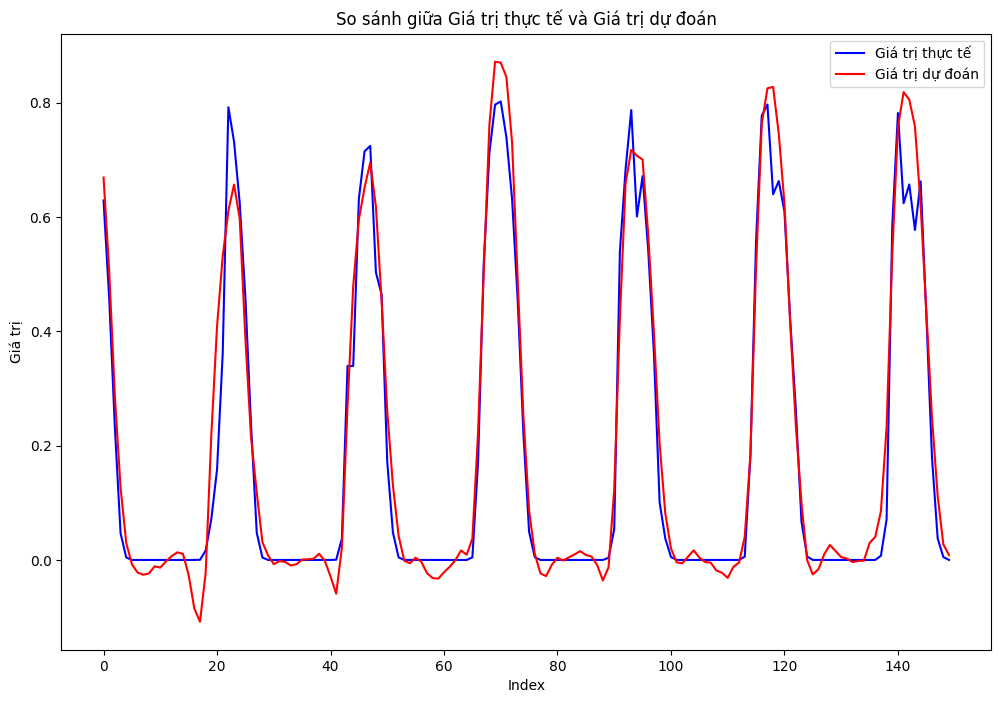
\includegraphics[width=0.3\textwidth]{images/demo2.png}\label{fig:demo2}}
%     \hfil

\begin{figure}[ht!]
    \centering
    \begin{subfigure}[t]{0.46\textwidth}
        \centering
        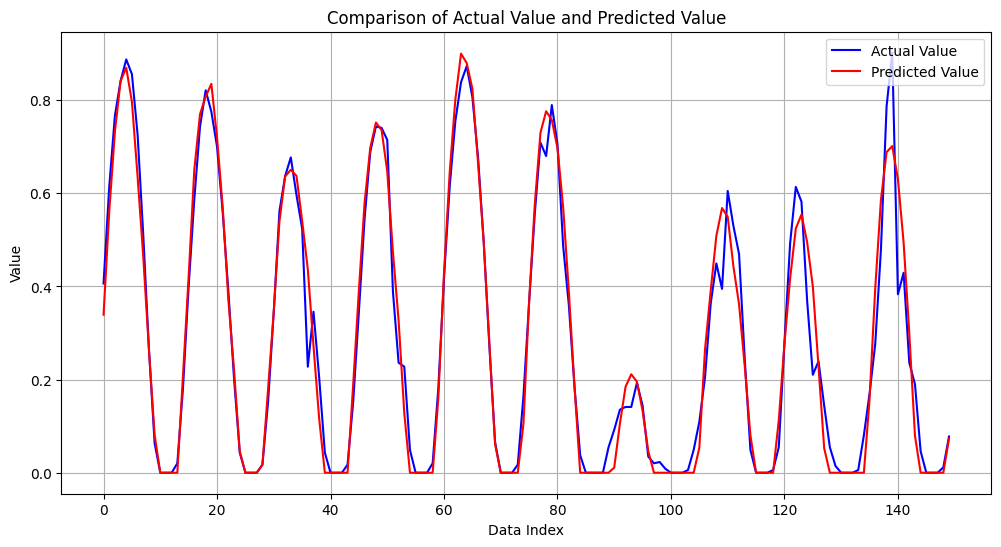
\includegraphics[width=\textwidth]{output2.png}
        \caption{Forecasting results of the TGNet on the competitive dataset}
        \label{fig:demo1}
    \end{subfigure}
    \hfill % Optional: add some horizontal space between the figures
    \begin{subfigure}[t]{0.45\textwidth}
        \centering
        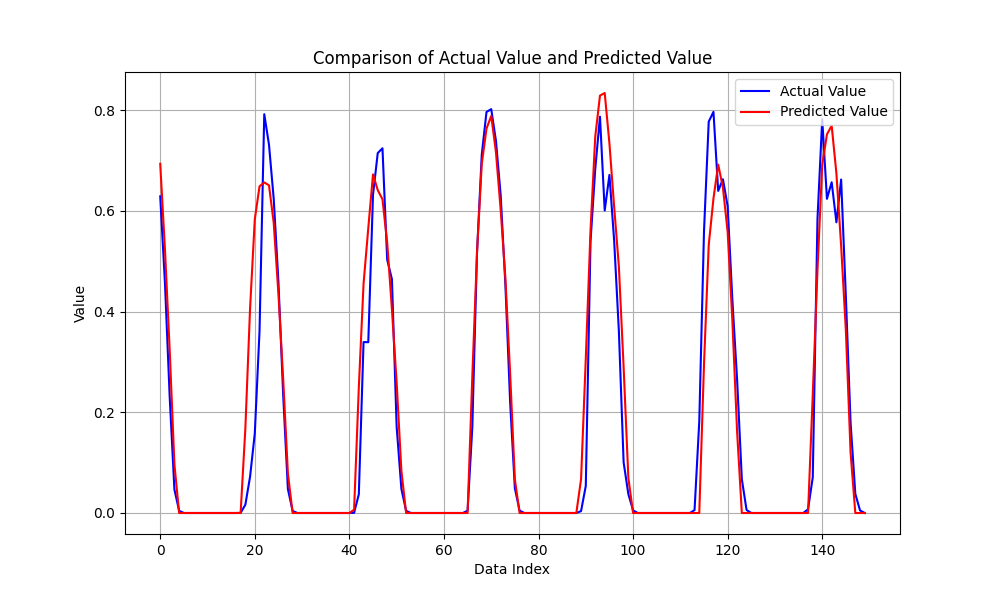
\includegraphics[width=\textwidth]{output3.png}
        \caption{Forecasting results of the TGNet on the GEFCom2014 dataset.}
        \label{fig:demo2}
    \end{subfigure}
    \caption{Comparison of forecasting results}
    \label{fig:predictions}
\end{figure}

\section{Conclusion and Discussion}\label{sec6}

This research introduces a hybrid framework for forecasting solar power generation that is suitable for implementation on edge devices. By effectively combining the temporal extraction functions of the Temporal Convolutional Network (TCN) with the sequential data handling capabilities of the Gated Regression Unit (GRU), this hybrid framework enhances the predictive performance for both short-term and long-term forecasts. Empirical evaluations conducted on two distinct datasets, namely the Competition Dataset and GEFCom2014, indicate that the proposed framework exhibits superior evaluation metrics in comparison to prevailing forecasting models. Moreover, the focus on edge computing deployment, employing sophisticated methodologies such as neural architecture search (NAS), quantization, and model pruning to minimize the parameter count while preserving high forecasting precision, illustrates the framework's versatility in edge computing contexts. Our forthcoming endeavors will involve the integration of supplementary data sources, including satellite imagery and localized meteorological data, to further refine forecasting accuracy and bolster the model’s adaptability across diverse environments.

%% The Appendices part is started with the command \appendix;
%% appendix sections are then done as normal sections
%% \appendix

%% \section{}
%% \label{}

%% References
%%
%% Following citation commands can be used in the body text:
%% Usage of \cite is as follows:
%%   \cite{key}         ==>>  [#]
%%   \cite[chap. 2]{key} ==>> [#, chap. 2]
%%

%% References with BibTeX database:

%\bibliographystyle{elsarticle-num}
\bibliography{ref}
%\bibliography{ref}
%% Authors are advised to use a BibTeX database file for their reference list.
%% The provided style file elsarticle-num.bst formats references in the required Procedia style

%% For references without a BibTeX database:

% \begin{thebibliography}{00}

%% \bibitem must have the following form:
%%   \bibitem{key}...
%%

% \bibitem{}

% \end{thebibliography}

\end{document}

%%
%% End of file `ecrc-template.tex'. 

 